\chapter{ACL.Test.Suite}
\section{AUnit} 
AUnit  3.4.0  ist ein Test-Framework, das f"ur Ada entwickelt worden ist.
Um AUnit innerhalb von GPS benutzen zu k"onnen, muss die
{\tt ADA\_PROJECT\_PATH}-Variable in der {\tt .bashrc} gesetzt werden
und auf den Pfad zeigen, wo die {\tt aunit.gpr}-Datei installiert
worden ist.  Im Normalfall d"urfte dieser Pfad auf einem Debian
''Squeeze'' (6.0) und im Allgemeinen Linux folgenderma"sen aussehen:
\\{\tt /usr/share/ada/adainclude}.  Dort wird standardm"a"sig auch die
  {\tt libaunit1-dev} von dem Paketmanager installiert.

Um sich in AUnit einzuarbeiten, gibt es eine Dokumentation und
Einf"uhrung ebenfalls von AdaCore namens AUnit
Cookbook\footnote{http://libre.adacore.com/wp-content/files/auto\_update/aunit-docs/aunit.html}.
Dort wird die Version 3.4.0 vorgestellt.  Des Weiteren gibt es ein
Videotutorial von Daniel
Bigelow \footnote{http://www.adacore.com/2010/05/11/aunit-tutorials/},
das in 7 Kapitel eingeteilt ist. Diese ist meiner Meinung nach nicht
sehr empfehlenswert, da es von schlechter Audioqualit"at ist, was das
Durcharbeiten stark erschwert.\\

Um die AUnit Library benutzen zu k"onnen, m"ussen folgende
Headerdateien eingebunden werden:
\begin{lstlisting}
with AUnit-Assertions; 
\end{lstlisting}
Der Aufbau von AUnit-1 f"ur Regressionstests ist folgenderma"sen gegliedert:
\begin{figure}[htp]
  \centering
  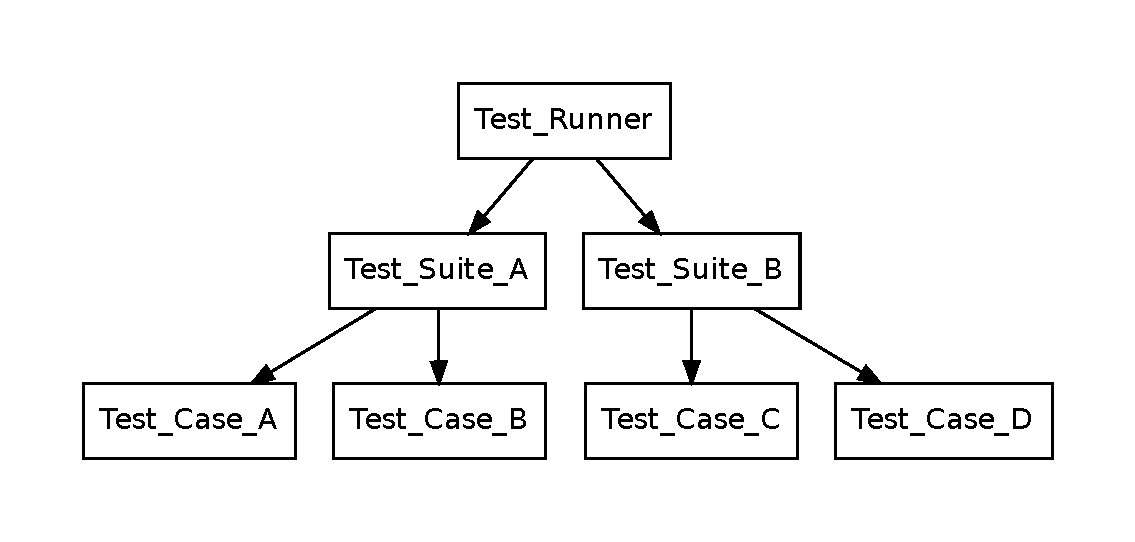
\includegraphics[scale=0.5,bb=0 0 385 567]{de/graph_aunit.pdf}
  \caption{Baumstruktur von AUnit}
\end{figure}
Es gibt eine Test-Case-Datei, in der die Tests f"ur eine
implementierte Operation enthalten sind.  Da es zum Beispiel f"ur die
Big Number sehr viele implementierte Grundoperationen gibt, die es zu
testen gilt, gibt es viele Test-Case-Dateien.  Unter anderem wurden
Test-Cases f"ur die Subtraktion wie auch die Addition angelegt.
Test-Suites enthalten einen Verbund an Test-Cases.  Die Test-Suites
werden wiederum in einem Test-Runner geb"undelt.  Dies ist die zu
kompilierende Datei und das daraus entstandene Programm vollf"uhrt
alle eingebeundenen Tests.  Dieses Verfahren macht es m"oglich, nur
die zu dem ver"anderten Quellcode zugeh"origen Regressionstests laufen
zu lassen.

Die Test-Cases innerhalb einer zu testenden Operation werden alle in
einer Prozedur namens {\tt Register\_Tests} eingtragen.  Beim Eintritt
in die Prozedur und beim Auftreten eines Fehlers innerhalb dieser kann
somit detailliert festgestellt werden, wo der Fehler aufgetreten ist
und mit welchen Testzahlen.

\begin{lstlisting}
procedure Register_Tests(T : in out Template_Test) is
  use Test_Cases.Registration;
     begin
      Register_Routine(T, Template_Test1'Access,"Template");
 end Register_Tests;
\end{lstlisting}

Des Weiteren enthalten die Test-Case-Dateien eine namensgebende
Prozedur, welche f"ur die "ubergeordnete Struktur der Test-Case-Datei
eine Rolle spielt.  Der in folgender Prozedur eingetragene Name

\begin{lstlisting}
function Name(T : Template_Test) return String_Access is
	begin
	   return new String'("Template Test");
	end Name;
\end{lstlisting}

ist der "ubergeordnete Name, der f"ur alle Prozeduren der
Test-Case-Datei Anwendung findet.

Ein Template-Test-Beispiel:
\begin{lstlisting}
procedure Template_Test1(T: in out Test_Cases.Test_Case'Class) is
      use AUnit.Assertions; 
   begin      
       Assert(A = B, "Failed with A and B.");
   end Template_Test1;
\end{lstlisting}

Wenn A und B entgegen der Erwartungen ungleich sind, wird ein
Fehlermeldung angezeigt. Ebenfalls wird der Name der Test-Case-Datei
und der Name der Prozedur ausgegeben.  Um zu bestimmen mit welchen
Testzahlen der Fehler aufgetreten ist, werden diese bei Fehlschlagen
des Tests parallel mit ausgegeben.

\section{GCOV}
{\tt gcov} ist ein Test Coverage Program, welches die Codeabdeckung
von Tests anzeigen kann und somit ein angenehmes Werkzeug ist, um
toten Code zu entdecken und herauszufinden, welche Codefragmente die
geschriebenen Tests abdecken.  Dieses Werkzeug wurde benutzt, um
sicher zu stellen, dass die Regressionstests eine Codeabdeckung von
100\% erreichen.  {\tt gcov} muss "uber den Paketmanager installiert
werden und wird "uber Flags w"ahrend des Kompilierens eingebunden.
Die Flags sind im Makefile der Regressionstests bereits vorhanden. Um
{\tt gcov} zu aktivieren m"ussen lediglich die gekennzeichneten
Kommentarzeichen entfernt werden.  Danach muss mit {\tt make gcov}
kompiliert werden und die resultierende ausf"uhrbare Datei ausgef"uhrt
werden.  Im Anschluss muss folgende Zeile ausgef"uhrt werden: {\tt
  gcov <filename>} (z.B. {\tt gcov
  test-big\_number\_add\_mod\_utils}).  Es wird eine Log-Datei mit der
Endung {\tt .gcov} generiert, in der alle nicht durchlaufenen Zeilen
des Codes mit Rauten (\#) gekennzeichnet sind und die Zeilen, die
durchlaufen worden sind mit einer Zahl, die die H"aufigkeit des
Eintritts in diese Zeile angibt.  Es k"onnen auch mehrere Dateien
(sogenannte ''graph files'' mit den Endungen {\tt *.gcno} und {\tt
  *.gcda}) in die resultierende Log-Datei eingebunden werden, indem
folgendes Kommando ausgef"uhrt wird:\\ {\tt gcov <filename>
  ... <filename>}\\ Die Ausgabe sollte folgenderma"sen aussehen:

{\tt File 'test-sha1.ads'\\
Lines executed:100.00\% of 3\\
test-sha1.ads:creating 'test-sha1.ads.gcov'\\

File '../src/crypto-asymmetric-rsa.ads'\\
Lines executed:100.00\% of 8\\
../src/crypto-asymmetric-rsa.ads:creating\\ 'crypto-asymmetric-rsa.ads.gcov'\\

File '../src/crypto-asymmetric-rsa.adb'\\
Lines executed:65.36\% of 179\\
../src/crypto-asymmetric-rsa.adb:creating\\ 'crypto-asymmetric-rsa.adb.gcov'\\}

Die erste Zeile zeigt die durchlaufene Datei, die zweite Zeile die
Prozentabdeckung der Datei und danach die Menge der ausfuehrbaren
Zeilen der Datei. Die letzte Zeile ist nur ein Hinweis, dass die
log-Datei mit der Endung {\tt .gcov} angelegt wird.  Eine log-Datei
kann folgenderma"sen aussehen:
\begin{lstlisting} 
14:   70:   procedure Set_Most_Significant_Bit(X: in out Big_Unsigned) is
 -:   71:   begin
14:   72:      X.Last_Index := Max_Length;
14:   73:      X.Number(Max_Length) := X.Number(Max_Length) or
 -:   74:        Shift_Left(Mod_Type(1), Mod_Type'Size-1);
14:   75:   end Set_Most_Significant_Bit; 
	    pragma Inline(Set_Most_Significant_Bit);
\end{lstlisting}

Die erste Zahlenreihe gibt an, wie oft die Zeile von einem Test
durchlaufen worden ist und die zweite Zahlenreihe ist die
Codezeilennummerierung der Originalsourecode-Datei.  Rauten (\#)
bedeuten, dass die Zeile von den Tests nicht durchlaufen wurde.

Die momentane Codeabdeckung ist teilweise aus der folgenden Tabelle zu
entnehmen:
\begin{figure}[htp]
\centering
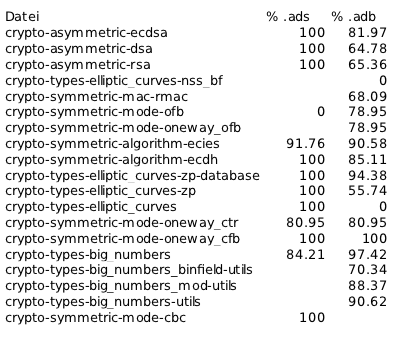
\includegraphics[scale=0.5,bb=0 0 385 567]{tabelle_gcov.png}
\caption{}
\label{}
\end{figure}

F"ur weitere Informationen, siehe http://gcc.gnu.org/onlinedocs/gcc/Gcov.html.
\chapter{Regressionstests}

Als minimalistische Vorlage f"ur Test-Cases gibt es die Dateien {\tt test-template.ad[s,b]} in dem Ordner {\tt test}.

\begin{lstlisting}
	with AUnit.Assertions; 
	with AUnit.Test_Cases.Registration;
	with Crypto.Types.Big_Numbers;
	with Big_Number_Constants;

\end{lstlisting}


Es werden die erforderlichen Pakete von AUnit und der ACL eingebunden wie auch die {\tt Big\_Number\_Constants}, welche alle Testkonstanten enth"alt.\\
Um die mathematischen Grundoperationen der {\tt Crypto-Types-Big\_Numbers} benutzen zu k"onnen, m"ussen folgende Zeilen im Code enthalten sein:

\begin{lstlisting}
	
    package Big is new Crypto.Types.Big_Numbers(4096);
    	use Big;
    	use Big.Utils;

    	use Big_Number_Constants;
    	
\end{lstlisting}

Die Testzahlen bewegen sich zwischen 0 und 4096 Bit.
Die Variablen X\_4096 bis X\_582 bezeichnen die einzelnen Konstanten, die in der {\tt Big\_Number\_Constants} zu finden sind.\\

\begin{lstlisting}
    X_4096, X_4095, X_3812, X_2048, X_1025, X_1024,
    X_768, X_582, X_1, X_0: Big_Unsigned;
    X, Result: Big_Unsigned;
\end{lstlisting}

{\tt X\_4096} ist die gr"o"ste 4096 Bit gro"se Zahl mit $2^{4096} - 1$ und gleichzeitig Big\_Unsigned\_Last. {\tt X\_4095} ist mit $2^{4095}$ die kleinste 4096 Bit gro"se Zahl.
{\tt X\_3812} ist eine per Zufall generierte Testzahl zwischen 4096 und 2048 Bit.
{\tt X\_2048} ist 2048 Bit gro"s, {\tt X\_1024} ist die gr"o"ste 1024 Bit gro"se Zahl und {\tt X\_1025} ist die kleinste 1025 Bit gro"se Zahl.
{\tt X\_768} und {\tt X\_582} sind ebenfalls per Zafall generierte Testzahlen wischen 1024 und 0 Bit.
Als weitere Testzahlen wurden 1 und 0 Bit verwendet.

Die Konstanten werden folgenderma"sen instanziiert:

\begin{lstlisting}
procedure Constants is
   begin
      X_4096 := To_Big_Unsigned(Cons_4096);
      X_3812 := To_Big_Unsigned(Cons_3812);
      X_1025 := To_Big_Unsigned(Cons_1025);
      X_1024 := To_Big_Unsigned(Cons_1024);
      X_768  := To_Big_Unsigned(Cons_768);
      X_1 := To_Big_Unsigned("1");
      X_0 := To_Big_Unsigned("0");
   end Constants;
\end{lstlisting}

Die {\tt Crypto-Types-Big\_Number} enth"alt die
Basisvergleichsoperationen Subtraktion, Addition, Division,
Multiplikation, die bin"are XOR-Verkn"upfung, AND-Verkn"upfung und
OR-Verkn"upfung, die Potenzierung und die Modulooperation.  Alle diese
Basisoperationen werden in den Test-Case-Dateien der {\tt
  Test-Suite\_Big\_Number} getestet.\\ Daneben gibt es noch die {\tt
  Crypto-Types-Big\_Numbers-Utils}, welche die Funktionen {\tt Swap,
  Set\_Least\_Significant\_Bit, Set\_Most\_Significant\_Bit, Is\_Odd,
  Is\_Even, Increase, Decrease, Shift\_Left, Rotate\_Left,
  Shift\_Right,\\ Rotate\_Right, Get\_Random, Bit\_Length,
  Lowest\_Set\_Bit, Length\_In\_Bit, Length\_In\_Byte, Greatest Common
  Divisor, Short\_Div, Big\_Div} und Konvertierungsfunktionen f"ur
{{\tt Big\_Unsigned, Mod\_Types, Bytes} und {\tt Strings}
  enth"alt.\\ Au"serdem gibt es die Ausgabefunktionen f"ur {\tt
    Big\_Unsigned}.  Danach folgt die {\tt
    Crypto-Types-Big\_Number-Mod\_Utils}, wo alle Grundoperationen mit
  der Modulooperation verkn"upft werden.  Des Weiteren enth"alt diese
  Bibliothek Funktionen wie {\tt Is\_Prime, Looks\_Like\_A\_Prime,
    Get\_Random} und den {\tt Miller\_Rabin\_Test}, welche aber noch
  ineffizient und rechenintensiv programmiert sind.\\ Danach folgen
  die Binfield\_Utils, welche die Grundoperationen im Gaulois-K"orper
  enthalten.\\

Die Tests f"ur die {\tt Big\_Number}-Bibliothek sind in der {\tt
  test\_suite\_big\_number.adb} gesammelt.\\ Um nur die Tests f"ur die
{\tt Big\_Number} ausf"uhren zu k"onnen, reicht es, die {\tt
  test-big\_number.adb} zu kompilieren und auszuf"uhren.  F"ur die
anderen Suites gilt "Ahnliches.  Im folgenden Diagramm sind die
Abh"angigkeit zu erkennen:

\begin{figure}[htp]
\centering
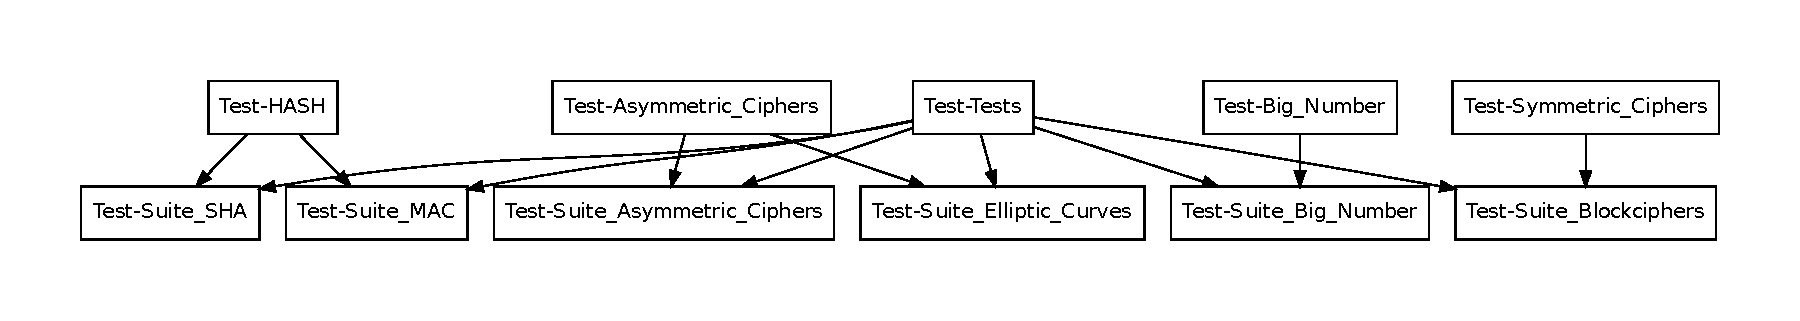
\includegraphics[scale=0.5,bb=0 0 385 567]{graph_suites.pdf}
\caption{Baumstruktur der Test-Suites}
\label{}
\end{figure}

Um die Test-Runner zu "andern, muss das Makefile ge"andert werden.
Um die einzelnen Test-Runner zu aktivieren, m"ussen die Kommentarzeichen im Makefile entfernt oder wahlweise gesetzt werden.\\

Im Anhang sind die Log-Dateien von {\tt gcov} zu finden, die die Code-Abdeckung enthalten.

\chapter{To Do}

Mehr Test-Cases f"ur die Big Number entwickeln und eventuell die
vorhandenen Tests "uberarbeiten.\\ Dasselbe gilt f"ur alle anderen
Test-Runner und Test-Cases.\\ Die Dokumentation der ACL
verbessern.\\ Die Regressionstests von AUnit-1 in AUnit-3.4
"ubersetzen.\\ Mit AUnit-3.4 Exceptiontests schreiben und
einf"ugen.\\ Die Pfadabdeckung analysieren.\\
